\chapter{Design Decisions and Justification}
\label{chap:4}

\section{Platform and Target Device}
\label{sec:4.1}

A constraint rather than a decision, stated first because every figure in the chapter depends on it.

The platform is Android: the development environment is Windows and an iOS build needs a macOS toolchain that is not available. The device is the Samsung Galaxy Z Flip5 named in 1.4.1, read from the handset with \texttt{adb shell \allowbreak{}getprop} rather than from a specification sheet. It was not selected against alternatives. It is the handset this project had, which 3.5.1 records as C1, and every figure below describes it and no other.

An emulator is useful during development and is not a target, because it measures neither real camera behaviour nor thermal throttling, the two unknowns the measurement exists to resolve.

\section{Pose Estimation Engine}
\label{sec:4.2}

Pose estimation sets the ceiling for everything after it: a joint absent from the model's output cannot be observed by any rule downstream.

\textbf{Latency decides, and it decides twice.} NFR-P3 bounds the 95th percentile of the per-frame path at 65 ms, and NFR-P2 sets a frame-rate floor of 22 fps, which 3.4.1 derives from the confirmation window. The second reaches further, because that window is counted in frames rather than milliseconds, so every frame per second buys response time as well as a smoother signal.

\textbf{Licence is a product constraint rather than a formality.} A copyleft licence that propagates to the application is a decision taken now whether or not it is noticed now.

\textbf{Topology is headroom, not a requirement.} The COCO seventeen-keypoint layout stops at the ankle, with no heel and no toe, and all six faults this project retains are expressible in it. It eliminates nothing here, and 4.6 is what makes the headroom matter.

\subsection{Shortlisting on published evidence}
\label{sec:4.2.1}

{\footnotesize
\setlength{\LTpre}{6pt}\setlength{\LTpost}{8pt}
\begin{longtable}{>{\raggedright\arraybackslash}p{\dimexpr 0.170\textwidth-2\tabcolsep\relax}>{\raggedright\arraybackslash}p{\dimexpr 0.257\textwidth-2\tabcolsep\relax}>{\raggedright\arraybackslash}p{\dimexpr 0.242\textwidth-2\tabcolsep\relax}>{\raggedright\arraybackslash}p{\dimexpr 0.198\textwidth-2\tabcolsep\relax}>{\raggedright\arraybackslash}p{\dimexpr 0.133\textwidth-2\tabcolsep\relax}}
\caption{Pose engines shortlisted on published evidence}\\
\toprule
Engine & Topology & Licence & Android integration & Model swappable \\
\midrule
\endfirsthead
\toprule
Engine & Topology & Licence & Android integration & Model swappable \\
\midrule
\endhead
\bottomrule
\endfoot
\bottomrule
\endlastfoot
Media\allowbreak{}Pipe Pose Landmarker & 33 landmarks, heel and foot index included & Apache 2.0 & First-class Tasks API & Yes \\
MoveNet & 17, COCO & Apache 2.0 & TFLite, with a sample application & Yes \\
RTMPose & 17 COCO, 26 in the Halpe variant & Apache 2.0 & ncnn export plus glue code & Yes \\
YOLO-pose & 17, COCO & AGPL-3.0, or a paid commercial licence & Export path required & Yes \\
ML Kit Pose Detection & 33 landmarks & Proprietary, free to use & Lowest, through Play Services & No \\
\end{longtable}
}

Published performance figures exist for some of these and are not used to choose. The BlazePose figure is over 30 frames per second on a Pixel 2 (Bazarevsky et al., 2020)\cite{bazarevsky2020blazepose}, and the MoveNet figures are latency on a Pixel 5 (TensorFlow Blog, MoveNet, 2021)\cite{tensorflow2021movenet}. Neither device is the handset this project targets, so those figures establish feasibility, which 2.3.1 covers, and not a choice on this handset.

Three options fall on the table above. \textbf{YOLO-pose} carries a licensing risk and offers nothing over the survivors, so the risk buys nothing. \textbf{RTMPose} needs an ncnn export and glue, and the deployability of its 26-keypoint variant here is unverified: a research task standing where a dependency should be. \textbf{ML Kit} publishes no latency figures, no accuracy figures and no way to substitute the model, and a system whose claim is that its behaviour can be checked cannot rest its perception layer on one that publishes nothing about its own. It is kept as a fallback.

Nothing on the table separates MediaPipe from MoveNet, so deciding between them on inspection would be deciding on preference. Both were measured on the target device, in the same harness, in one run.

\subsection{How the engines were measured}
\label{sec:4.2.2}

Appendix A describes the instrument, lists every run and gives the caveats. Three points bear on the table below.

\textbf{The harness runs the engine, not the product.} It has no constraint evaluation, no trigger policy and no audio, so NFR-P1 cannot be obtained from it at all and the comparison against NFR-P3 is favourable to the pipeline by whatever the missing stages cost.

\textbf{The device was not cold.} Battery temperature climbed from 34.1 C at the start of the sweep to a peak of 39.0 C, so a configuration measured late began warmer than one measured early. Here that runs against the winner.

\textbf{An earlier sweep measured a client defect and is superseded.} It put frame preparation at 44 ms against an allocation of 15. That was not the engine: the analyzer was rotating each frame in software when the engine accepts the rotation as a parameter. Removing it cut median preparation to 10 ms on the identical MediaPipe Lite GPU configuration, left median inference at 50 ms against 52, and took its frame rate from 17.70 to 29.84. An engine comparison taken while a fixed per-frame tax dominated every row would have been a comparison of the tax.

\subsection{What the measurement says}
\label{sec:4.2.3}

{\tiny
\setlength{\LTpre}{6pt}\setlength{\LTpost}{8pt}
\begin{longtable}{>{\raggedright\arraybackslash}p{\dimexpr 0.136\textwidth-2\tabcolsep\relax}>{\raggedright\arraybackslash}p{\dimexpr 0.117\textwidth-2\tabcolsep\relax}>{\raggedright\arraybackslash}p{\dimexpr 0.098\textwidth-2\tabcolsep\relax}>{\raggedright\arraybackslash}p{\dimexpr 0.138\textwidth-2\tabcolsep\relax}>{\raggedright\arraybackslash}p{\dimexpr 0.152\textwidth-2\tabcolsep\relax}>{\raggedright\arraybackslash}p{\dimexpr 0.126\textwidth-2\tabcolsep\relax}>{\raggedright\arraybackslash}p{\dimexpr 0.136\textwidth-2\tabcolsep\relax}>{\raggedright\arraybackslash}p{\dimexpr 0.097\textwidth-2\tabcolsep\relax}}
\caption{The engine comparison as measured on the target device}\\
\toprule
Engine & Delegate & Frames per second & Inference, median & Preparation, median & Total, 95th percentile & Knee jitter & Battery at start \\
\midrule
\endfirsthead
\toprule
Engine & Delegate & Frames per second & Inference, median & Preparation, median & Total, 95th percentile & Knee jitter & Battery at start \\
\midrule
\endhead
\bottomrule
\endfoot
\bottomrule
\endlastfoot
Media\allowbreak{}Pipe Lite & CPU & 27.61 & 80 ms & 9 ms & 107 ms & not measured & 34.1 C \\
Media\allowbreak{}Pipe Lite & GPU & 29.84 & 50 ms & 10 ms & 71 ms & 0.00045 & 35.9 C \\
Media\allowbreak{}Pipe Full & CPU & 18.29 & 104 ms & 11 ms & 137 ms & 0.00040 & 36.9 C \\
Media\allowbreak{}Pipe Full & GPU & 29.85 & 55 ms & 11 ms & 76 ms & 0.00028 & 37.1 C \\
Media\allowbreak{}Pipe Heavy & CPU & 5.86 & 225 ms & 12 ms & 262 ms & 0.00045 & 37.7 C \\
Media\allowbreak{}Pipe Heavy & GPU & 23.99 & 91 ms & 11 ms & 124 ms & 0.00024 & 38.2 C \\
MoveNet Lightning & CPU & 26.89 & 20 ms & 7 ms & 36 ms & 0.00066 & 39.0 C \\
MoveNet Lightning & GPU & 29.57 & 13 ms & 7 ms & 27 ms & 0.00111 & 38.5 C \\
\end{longtable}
}

The deciding sweep, on the device in 4.1, in the order printed, 60 measured seconds each at 720 by 1280. Appendix A names the run and holds its data. Total is preparation plus inference for one frame, the quantity NFR-P3 bounds at 65 ms. Jitter is the mean frame-to-frame movement of the knee with the subject still, in normalised units, and measures how quiet the model is rather than how accurate it is.

\textbf{One row is not a result.} The harness recorded that the framing gate timed out on MediaPipe Lite CPU and that it ran without a confirmed subject, and its knee detection rate is zero. Its timing columns measure the engine on an empty scene; its landmark columns measure nothing. It is printed with the gap visible, and at 107 ms it misses NFR-P3 by 42 ms whatever was in front of the camera.

\textbf{Frame rate no longer separates the top of the table.} Four configurations sit between 26.89 and 29.85 fps, which is the camera's 30 fps ceiling rather than a property of any model. In the superseded sweep nothing reached it and frame rate was the discriminator; here it is saturated, and what matters is the latency headroom underneath.

\textbf{Two configurations meet NFR-P3 and both are MoveNet}, at 27 ms on the GPU and 36 ms on the CPU. The best MediaPipe configuration is Lite on the GPU at 71 ms, and Full, Heavy and the two CPU variants follow at 76, 124, 137 and 262.

\textbf{MediaPipe Lite on the GPU straddles the bound rather than failing it.} The same configuration and build returned 60 ms on a cold device in an earlier run, 71 ms at 35.9 C here, and 79 ms at 36.8 C immediately afterwards. The engine is not inconsistent; the device is warm. A configuration whose compliance depends on the handset being cold complies at the start of a session and not at minute ten, which is what NFR-P4 exists to catch. MoveNet on the GPU has 2.4 times the bound in hand, and it ran last at 38.5 C, warmer than every MediaPipe row, so the thermal confound favours the loser.

\textbf{What MoveNet gives up is jitter.} The knee moves 0.00111 of a normalised unit per frame with the subject still against 0.00045 for MediaPipe Lite on the GPU, making MoveNet the noisiest model in the table by 2.5 times. Two assumptions turn that into judgeable units and neither is firm: the metric is a straight-line distance in coordinates that 6.2.1 shows are not a length, giving 0.8 pixels horizontally and 1.4 vertically, and the angle conversion needs a femur length the record does not store, taken at 256 pixels. The result is roughly 0.3 degrees of knee angle per frame, an order of magnitude under the 6 and 10 degree thresholds it has to support, and that holds with both assumptions wrong by a factor of two.

\textbf{Decision. MoveNet Lightning, on the GPU delegate.} Over MoveNet on the CPU on latency headroom, 27 ms against 36, which leaves more of the handset free for the rest of the pipeline. Over every MediaPipe configuration because none meets the requirement on a warm device.

\subsection{The engine was checked before it was trusted}
\label{sec:4.2.4}

The adapter between the output tensor and the assessment layer is written by hand, and MoveNet emits each keypoint as row, column and score rather than x, y and score. Read in the obvious order, that transposes every landmark while leaving every value inside its valid range, which is a system that fails silently.

The check is agreement with the engine being replaced. Over four 60-second runs of a subject standing still, three on MoveNet and one on MediaPipe Lite on the GPU, every MoveNet knee median fell within 0.035 of frame width and 0.015 of frame height of where MediaPipe put the same joint, with left and right on the correct sides. A transposed axis would have moved a knee by several tenths. Appendix A names the four runs, and the medians are in their per-frame files.

This rules out a class of integration defect and nothing more. There is no ground truth in it, so both engines could be wrong together. The subject also stood between runs instead of holding one position, so part of the disagreement is the subject.

\subsection{What this run does not settle}
\label{sec:4.2.5}

\textbf{NFR-P4 is not answered by this sweep.} Sixty seconds cannot show a thermal limit that arrives in the ninth minute, and at the time this comparison was made the only ten-minute runs on record were on MediaPipe, before the preparation fix. 9.4.1 reports a ten-minute run on the configuration this sweep chose.

\textbf{The jitter has a known cost and it was paid once already.} The segmenter tests whether the rep driver has stopped moving in order to name the bottom of a movement, and that threshold had been set at 0.05 degrees per frame against MediaPipe. MoveNet's noise floor at the knee is six times that, so the test could never be satisfied and the phase it gates was never entered: a recorded set of ten deliberately shallow squats raised nothing at all. A threshold calibrated against one engine's noise is a hidden dependency on that engine, and swapping the engine exposed it where failure was silent.

\textbf{The jitter columns compare two scores that are not the same quantity.} The harness counts a knee as present at a fixed floor of 0.5, while MediaPipe reports a visibility and MoveNet a keypoint heatmap score; on the same standing pose the knee scored 0.986 under one and 0.761 under the other. Both cleared the floor standing, so the reading here holds, but it would not in a flexed position where MoveNet's score falls further.

\textbf{Nothing here measures angular accuracy.} Jitter is repeatability with the subject still, not correctness. The choice is supported on everything measured and untested on that axis, which is the position 4.5.4 records for the thresholds.

\textbf{The comparison is between two engines, not five.} The other three were eliminated in 4.2.1 on licence, integration cost and disclosure, none of which a benchmark would have changed.

\textbf{What would reverse it.} A ten-minute run showing MoveNet losing the frame-rate floor under sustained load, which would promote MediaPipe Lite on the GPU and make NFR-P3 unmeetable on this handset. Or the landmark noise proving to change a verdict on recorded sets, which reopens the decision with MediaPipe Full on the GPU at a cost of 49 ms of 95th-percentile latency.

\section{Client and Backend Stack}
\label{sec:4.3}

Three questions settled together because they are one argument: what the client is written in, what runs where, and what the server is for. The hot path is a per-frame pipeline sustained for minutes, and every abstraction between the camera and the pose engine costs a buffer copy or a serialisation step inside a loop that 3.4.1 shows has no room.

\subsection{Client framework}
\label{sec:4.3.1}

{\footnotesize
\setlength{\LTpre}{6pt}\setlength{\LTpost}{8pt}
\begin{longtable}{>{\raggedright\arraybackslash}p{\dimexpr 0.233\textwidth-2\tabcolsep\relax}>{\raggedright\arraybackslash}p{\dimexpr 0.217\textwidth-2\tabcolsep\relax}>{\raggedright\arraybackslash}p{\dimexpr 0.234\textwidth-2\tabcolsep\relax}>{\raggedright\arraybackslash}p{\dimexpr 0.176\textwidth-2\tabcolsep\relax}>{\raggedright\arraybackslash}p{\dimexpr 0.140\textwidth-2\tabcolsep\relax}}
\caption{Client frameworks compared}\\
\toprule
Criterion & Native Kotlin & Flutter & React Native & Unity \\
\midrule
\endfirsthead
\toprule
Criterion & Native Kotlin & Flutter & React Native & Unity \\
\midrule
\endhead
\bottomrule
\endfoot
\bottomrule
\endlastfoot
Direct camera frame access & CameraX, first class & Through a channel, a copy per frame & Through a native module & Indirect \\
TFLite support on Android & First-class, the reference runtime & Community bindings & Community bindings & Limited \\
Overhead inside the per-frame path & None & A bridge crossing per frame & A bridge crossing per frame & Engine overhead \\
Control of the GPU delegate & Direct & Indirect & Indirect & Indirect \\
Benefit from being cross-platform & Not applicable & Unrealised & Unrealised & Unrealised \\
Interface capability for this product & Sufficient, with Compose & Strong & Strong & More than needed \\
\end{longtable}
}

\textbf{Decision. Native Android in Kotlin: CameraX for capture, TFLite for pose, Jetpack Compose for the interface, and one JSON file per set for the local store.}

The cross-platform options are rejected on one sufficient ground. Their principal benefit is serving iOS, which 4.1 excluded, while their principal cost is a bridge crossing inside the one path with a hard deadline. That is not a trade-off; it is one side of a trade with nothing on the other.

\subsection{Where the computation runs}
\label{sec:4.3.2}

{\footnotesize
\setlength{\LTpre}{6pt}\setlength{\LTpost}{8pt}
\begin{longtable}{>{\raggedright\arraybackslash}p{\dimexpr 0.200\textwidth-2\tabcolsep\relax}>{\raggedright\arraybackslash}p{\dimexpr 0.104\textwidth-2\tabcolsep\relax}>{\raggedright\arraybackslash}p{\dimexpr 0.270\textwidth-2\tabcolsep\relax}>{\raggedright\arraybackslash}p{\dimexpr 0.184\textwidth-2\tabcolsep\relax}>{\raggedright\arraybackslash}p{\dimexpr 0.242\textwidth-2\tabcolsep\relax}}
\caption{Where the computation runs: four placements compared}\\
\toprule
Criterion & All on device & Pose on device, assessment on a server & Frames streamed to a server & On device, records synchronised \\
\midrule
\endfirsthead
\toprule
Criterion & All on device & Pose on device, assessment on a server & Frames streamed to a server & On device, records synchronised \\
\midrule
\endhead
\bottomrule
\endfoot
\bottomrule
\endlastfoot
Satisfies NFR-P1 & Yes & No, the network is in the loop & No & Yes, the network is never in the loop \\
Image data leaves the device & No & No, landmarks only & Yes & No \\
Works with no connectivity & Yes & No & No & Yes, fully \\
History survives the device & No & Partly & Yes & Yes \\
Running cost per user & None & Per session & High & Per synchronisation \\
Load on the handset & Highest & Lower & Lowest & Highest \\
\end{longtable}
}

The two middle options fail on the first row structurally rather than as a matter of tuning: a network round trip inside a 300 ms budget cannot be made reliable over mobile data, and NFR-S3 is lost with it. The first and last differ on one row only, and keeping everything local loses the history with the phone, so a trainee who changes handsets after a year loses the year and FR-18 does not hold.

\textbf{Decision. The live path runs entirely on the device. Session records synchronise to a server-side profile when a connection exists and the trainee is signed in.} The network is used between sets and after them, never during one, and what crosses it is the derived list in FR-22 and nothing else.

\subsection{The server}
\label{sec:4.3.3}

The phase 1 server has one job: hold the profile and the session history, and reconcile them with a device that may have been offline for a week.

\textbf{Decision. A single FastAPI service in Python over SQLite.} The workload that follows this phase is language-model orchestration, retrieval and a safety test suite, which is where the Python ecosystem is strongest, so choosing it now costs nothing and avoids a rewrite at the boundary.

\textbf{What this costs.} The whole compute load sits on the handset, which is the thermal risk 4.1 recorded, and nothing in this phase provides remote diagnostics, so a failure on a user's device cannot be investigated remotely.

\textbf{What would reverse it.} iOS entering scope. Or the handset proving unable to carry the load within its thermal envelope, which would force assessment onto the server and reopen 4.4 with it.

\section{Immediate Feedback Path}
\label{sec:4.4}

The product claim in 1.2 is a correction that arrives inside the repetition. 3.4.1 turns that into 300 ms from fault to first audible sample, of which 60 ms is allocated to getting sound out of the device.

A language model cannot fit that allocation.

{\small
\setlength{\LTpre}{6pt}\setlength{\LTpost}{8pt}
\begin{longtable}{>{\raggedright\arraybackslash}p{\dimexpr 0.381\textwidth-2\tabcolsep\relax}>{\raggedright\arraybackslash}p{\dimexpr 0.210\textwidth-2\tabcolsep\relax}>{\raggedright\arraybackslash}p{\dimexpr 0.409\textwidth-2\tabcolsep\relax}}
\caption{The cost assumed for each stage of the immediate feedback path}\\
\toprule
Stage & Assumed cost & Basis \\
\midrule
\endfirsthead
\toprule
Stage & Assumed cost & Basis \\
\midrule
\endhead
\bottomrule
\endfoot
\bottomrule
\endlastfoot
Network round trip & 50 to 300 ms & Mobile data, variable, occasionally much worse \\
Time to first token & 200 to 800 ms & A hosted model, typical range \\
Generation to the end of a short utterance & 200 to 600 ms & Streamed \\
Synthesis and the start of playback & 200 to 500 ms & Cloud or on-device speech \\
Total & roughly 0.65 to 2.2 s &  \\
\end{longtable}
}

\textbf{None of these is a measurement.} They are assumptions, recorded so the reasoning can be inspected, as 3.5.1 C5 requires. The argument does not depend on their precision: the optimistic end consumes most of a repetition and the pessimistic end exceeds it entirely.

A second force has nothing to do with time. A generated utterance is not fixed in advance, so nothing guarantees the wording stays inside what the system can support, and for a product whose claim is that every cue traces to a published criterion, free generation in the live path contradicts the claim.

{\footnotesize
\setlength{\LTpre}{6pt}\setlength{\LTpost}{8pt}
\begin{longtable}{>{\raggedright\arraybackslash}p{\dimexpr 0.238\textwidth-2\tabcolsep\relax}>{\raggedright\arraybackslash}p{\dimexpr 0.131\textwidth-2\tabcolsep\relax}>{\raggedright\arraybackslash}p{\dimexpr 0.197\textwidth-2\tabcolsep\relax}>{\raggedright\arraybackslash}p{\dimexpr 0.185\textwidth-2\tabcolsep\relax}>{\raggedright\arraybackslash}p{\dimexpr 0.249\textwidth-2\tabcolsep\relax}}
\caption{Four ways to produce a spoken cue, compared}\\
\toprule
Criterion & Hosted language model & On-device language model & Pre-authored cue bank & Template plus synthesis at playback \\
\midrule
\endfirsthead
\toprule
Criterion & Hosted language model & On-device language model & Pre-authored cue bank & Template plus synthesis at playback \\
\midrule
\endhead
\bottomrule
\endfoot
\bottomrule
\endlastfoot
Worst-case fault to audio & Fails the allocation & Unknown, likely marginal & Bounded: a lookup and playback & Bounded by synthesis, longer than a lookup \\
Wording fixed in advance & No & No & Yes & Yes \\
Works with no network & No & Yes & Yes & Yes \\
Traceable to the fault taxonomy & Weak & Weak & By construction & Yes \\
Can say something outside its competence & Yes & Yes & No & No \\
Cost in the live path & Moderate & High, competes with pose inference & Negligible & Low \\
Cost to add a cue & None & None & Author and render one clip & Write one string \\
Adapts its phrasing to the user & Yes & Yes & No & No \\
\end{longtable}
}

The on-device model competes for the scarcest resource, which 4.1 records as the thermal risk, and synthesis at playback puts a variable cost inside a 60 ms allocation for no gain over a clip rendered once.

\textbf{Decision. A bank of pre-authored cues with pre-rendered audio, keyed by a discrete fault code. No language model takes part in the live path.}

The system is two-tier by design: the reflex tier fires on a confirmed fault and is a dictionary lookup and a cached clip, while the deliberative tier belongs to the second phase, runs between sets and has no hard deadline. With no network call, no generation and no synthesis in the live path, the allocation is met by construction rather than by optimisation.

\subsection{What a pre-rendered bank turned out to cost, and what it caught}
\label{sec:4.4.1}

Rendering the bank exposed a defect in the wording of the requirement. The synthesiser pads every utterance with silence before the first word, measured at 95 to 111 ms across the eight cues the bank held at the time. A file whose first sample is silent satisfies a requirement written as time to the first sample and fails the same requirement written as time to the first audible sample, and the difference is roughly a third of the whole budget, hidden inside a binary asset where no test would have found it. The lead-in is now cut when the bank is generated, keeping 8 ms so playback does not begin mid-waveform, and 3.4.1 specifies the audible sample for this reason.

\textbf{What this costs.} What the system says during a set is fixed when the cue is authored, with no adaptation to the trainee inside the repetition, and the audio ships in the bundle.

\textbf{What it buys, beyond the latency.} The complete set of sentences the system can ever say during a set is finite and reviewable before release. This was not the reason for the decision.

\textbf{What would reverse it.} Measurement showing an on-device model produces first audio inside the allocation with output constrained to the taxonomy. Or measurement showing even the cached path misses the allocation, which would force the trigger policy to fire earlier in the movement.

\section{Movement Assessment Approach}
\label{sec:4.5}

The assessment layer takes a stream of landmarks per frame, and 4.4 fixes its output: a discrete fault code from a closed set, plus a repetition count. A design emitting only a continuous quality score cannot key the lookup.

Four forces. \textbf{There is no labelled training data and no budget to produce it}, where a supervised classifier needs hundreds to thousands of labelled examples per fault per exercise. \textbf{Every cue must trace to a documented reason}, which is O5: a rule states its reason in its own text, a classifier states a probability. \textbf{The live path shares silicon with pose estimation}, which 4.1 flags as the scarce resource. And, cutting against the choice that follows, \textbf{a geometric rule is not free of data}: a depth rule needs a number to compare against, so the difference between the options is one of quantity, not of kind.

{\footnotesize
\setlength{\LTpre}{6pt}\setlength{\LTpost}{8pt}
\begin{longtable}{>{\raggedright\arraybackslash}p{\dimexpr 0.183\textwidth-2\tabcolsep\relax}>{\raggedright\arraybackslash}p{\dimexpr 0.186\textwidth-2\tabcolsep\relax}>{\raggedright\arraybackslash}p{\dimexpr 0.167\textwidth-2\tabcolsep\relax}>{\raggedright\arraybackslash}p{\dimexpr 0.217\textwidth-2\tabcolsep\relax}>{\raggedright\arraybackslash}p{\dimexpr 0.247\textwidth-2\tabcolsep\relax}}
\caption{Three approaches to movement assessment, compared}\\
\toprule
Criterion & Learned classifier over sequences & Declared geometric constraints & Hybrid: rules segment, a model classifies & Self-supervised, with a small supervised head \\
\midrule
\endfirsthead
\toprule
Criterion & Learned classifier over sequences & Declared geometric constraints & Hybrid: rules segment, a model classifies & Self-supervised, with a small supervised head \\
\midrule
\endhead
\bottomrule
\endfoot
\bottomrule
\endlastfoot
Labelled data required & Hundreds to thousands per fault & Tens of clips to set a threshold & High & Moderate, and expert-labelled \\
Available to this project & No & Yes & No & No \\
States why it fired & No, a probability & Yes, the violated constraint & Partly & No \\
Traceable to the taxonomy & Weak & By construction & Partly & Weak \\
Cost in the live path & Model inference per repetition & Arithmetic per frame & Model inference & Model inference \\
Deterministic and unit-testable & No & Yes & Partly & No \\
Cost of a new exercise & Retraining, and new labels & Authoring a specification & Retraining & Retraining \\
Handles subtle or compound faults & Better & Only what the geometry shows & Better & Best \\
Published precedent & Common & Pose Trainer, in 2.3.2 & Common & Fitness-AQA, in 2.3.2 \\
\end{longtable}
}

The second row decides it. Three options are stronger on the last row and all three are unavailable, because each needs a labelled corpus that does not exist here. Choosing one would mean either inventing labels or not evaluating the result.

\textbf{Decision. Movement assessment is geometric constraints over landmark trajectories, declared per exercise, with absolute thresholds that the system states and the user is measured against.}

\subsection{Where the standard comes from, since the user does not supply it}
\label{sec:4.5.1}

The alternative is a per-user reference measured before the first set, and this project built one before removing it. It answers a real objection: a trainee whose ankle mobility does not permit a full squat will be told to go deeper on every repetition by a system holding one number for everybody, and 3.4.3 records that a cue the user cannot act on is the most damaging failure this product has.

It is answered in the wrong place, for three reasons in order of weight.

\textbf{A product that asks the user what correct looks like has inverted its own premise.} The purpose in 1.1 is that the system knows what a correct repetition is and the user does not. A calibration step grades the user against their own demonstration, so a wrong demonstration becomes the standard and is confirmed on every set afterwards. The failure is silent and it is worst for exactly the users the product exists for.

\textbf{The published sources give absolute criteria}, so the calibration was discarding evidence the project already had. The Functional Movement Screen defines adequate squat depth as the femur below horizontal, a statement about the body and not about a particular body. Implemented literally, that is the hip landmark at or below the knee landmark.

\textbf{A fixed criterion removes a class of invented number.} A threshold expressed as an offset from a calibration needs both the procedure and the offset, and the offset has no source.

The objection the calibration was built for remains. The containment is not a softer threshold. It is a different response: a trainee who cannot reach the position should be told once, as an observation about mobility, instead of being cued every repetition. That path is specified and not built, and 9.5 records it as outstanding.

\subsection{A criterion is not a tolerance, and the difference is measured}
\label{sec:4.5.2}

A threshold of exactly zero would have the system speak about differences it cannot resolve. Ten squats performed at a deliberately constant depth gave a standard deviation of 0.0107 at the deepest point of each repetition and a range of 0.0163 either side of its centre. At zero, those ten split six passes to four faults, which is the measurement's own noise reported as a difference in the trainee's form.

The threshold is set 0.0209 below the criterion, at which all ten pass. The direction is the one 3.4.3 requires, since a false positive costs more than a missed fault. In degrees of femur angle that is about six, a conversion needing a femur length the recording does not store and which was taken at 256 pixels. \textbf{The threshold itself is in recorded units and does not depend on that assumption.}

Two further things this number is not. It is not from a source, and the specification records its threshold source as empty rather than citing the FMS for a tolerance the FMS does not give. And it mixes the trainee's variation between repetitions with the measurement's noise on an identical position, which this procedure cannot separate.

The same procedure sets the two hip thresholds in the push-up and the plank; 6.4.2 gives those distributions. The principle is that where a published criterion exists it is implemented directly, where a tolerance is needed it is measured and labelled as measured, and where neither exists the number is marked provisional in the file carrying it.

\subsection{Three things authoring the rules changed}
\label{sec:4.5.3}

\textbf{A published criterion can be a better design than the one it authorises.} Forward lean was first written as an absolute 45 degrees, which is wrong in a way worth recording: lean in a bodyweight squat is set largely by femur-to-torso proportion and ankle mobility, neither under the trainee's control, so a fixed angle fires constantly on a long-femured trainee squatting correctly and never on a short-limbed one genuinely over-pitching. The Functional Movement Screen compares the upper torso to the tibia within the same frame, which adapts to the body without asking the body anything.

\textbf{Each repetition has to be judged on its own, and the obvious implementation does not do that.} A fault evaluated over a set naturally tracks the most violating value seen so far, which is right for a deviation that can appear at any moment and wrong for one describing a repetition as a whole. A trainee who squats shallow five times and then once slightly deeper, still above the line, has performed six faulty repetitions; a running extreme reports the deepest and clears the rest. The format therefore distinguishes a fault judged continuously from one judged once per repetition, the second decided from samples collected within that repetition and discarded at its boundary.

\textbf{The declared camera view and the observable fault set are one decision rather than two.} A measurement taken along the axis the camera looks down is not available at any accuracy. Knee valgus is a frontal measurement while the squat declares a side view, where the two knees project to nearly the same point; the engine still returns the occluded side, but it is an inference, and a threshold on an inference fires at random. The fault was removed rather than approximated, as was push-up elbow flare, and both exclusions are recorded in the specification files themselves.

\subsection{What this approach cannot do}
\label{sec:4.5.4}

\textbf{The thresholds rest on one subject and one session.} Every source located establishes that a deviation is a fault and gives an observable condition for it; none gives the quantity at which the fault begins. The tolerances were measured on the author, performing the fault on purpose, in a single session per exercise. A deliberate fault is larger than one appearing under fatigue, so every detection rate derived from those recordings is an upper bound. The format records the taxonomy source and the threshold source as separate fields, and the threshold field is empty for every fault in the three files.

\textbf{The fault set has not been reviewed by a certified trainer.} The protocol is in 10.4: a trainer labels recorded sets without seeing the system's output or the author's own labels, and what the trainers set is what the report reports.

\textbf{Only geometrically observable faults can be detected.} Tempo, control and bracing are outside this method, and 2.2 shows they are outside the whole category rather than outside this choice alone.

\textbf{A trainee who cannot reach the standard is told so on every repetition}, which is the cost of removing the calibration and is not yet contained.

\textbf{Compound faults are not modelled.} Two simultaneous faults produce two codes, and the trigger policy decides which is spoken.

\textbf{What would reverse it.} An expert-labelled corpus becoming available, making the self-supervised option viable for faults the rules cannot separate. Or rules failing to separate a named fault from correct execution on recorded clips, which would require that fault to be removed with the removal stated rather than approximated.

\section{Exercise Extensibility Mechanism}
\label{sec:4.6}

O2 commits the system to adding an exercise without hand-written rules, and 2.4 is why it matters: no surveyed product discloses how an exercise is added at all. If a reviewer asks how the third exercise was added and the answer involves writing a class, the claim fails in public.

{\footnotesize
\setlength{\LTpre}{6pt}\setlength{\LTpost}{8pt}
\begin{longtable}{>{\raggedright\arraybackslash}p{\dimexpr 0.254\textwidth-2\tabcolsep\relax}>{\raggedright\arraybackslash}p{\dimexpr 0.193\textwidth-2\tabcolsep\relax}>{\raggedright\arraybackslash}p{\dimexpr 0.184\textwidth-2\tabcolsep\relax}>{\raggedright\arraybackslash}p{\dimexpr 0.216\textwidth-2\tabcolsep\relax}>{\raggedright\arraybackslash}p{\dimexpr 0.153\textwidth-2\tabcolsep\relax}}
\caption{Four extensibility mechanisms, compared}\\
\toprule
Criterion & A class per exercise & A declarative specification & An embedded scripting language & A model per exercise \\
\midrule
\endfirsthead
\toprule
Criterion & A class per exercise & A declarative specification & An embedded scripting language & A model per exercise \\
\midrule
\endhead
\bottomrule
\endfoot
\bottomrule
\endlastfoot
Adding an exercise requires code & Yes & No & Yes, script code & No, but it requires data \\
Readable by a non-programmer & No & Yes & No & No \\
Reviewable against the taxonomy & Hard, the logic is scattered & Yes, one file per exercise & Partly & No \\
Testable with no device & Partly & Yes, data in, codes out & Partly & No \\
Expressiveness & Unlimited & Bounded & High & High \\
Risk of divergence between exercises & High, each author improvises & Low, the schema constrains & Moderate & Not applicable \\
Available to this project & Yes & Yes & Yes & No, it needs labels \\
\end{longtable}
}

A class per exercise is what the category appears to do and is the thing O2 exists to avoid. A scripting language buys expressiveness this phase does not need and gives up reviewability.

\textbf{Decision. An exercise is added by authoring one declarative specification file. A single generic evaluator executes it, and the evaluator is the only code.}

{\small
\setlength{\LTpre}{6pt}\setlength{\LTpost}{8pt}
\begin{longtable}{>{\raggedright\arraybackslash}p{\dimexpr 0.253\textwidth-2\tabcolsep\relax}>{\raggedright\arraybackslash}p{\dimexpr 0.747\textwidth-2\tabcolsep\relax}}
\caption{What a specification file declares, block by block}\\
\toprule
Block & Contents \\
\midrule
\endfirsthead
\toprule
Block & Contents \\
\midrule
\endhead
\bottomrule
\endfoot
\bottomrule
\endlastfoot
\texttt{landmarks} & Which landmarks this exercise depends on \\
\texttt{rep\_\allowbreak{}driver} & One scalar signal, how it is extracted, and hysteresis bounds for segmentation \\
\texttt{phases} & Named intervals over that signal \\
\texttt{faults} & Per fault: a code, whether it is judged every frame or once per repetition, the phases it is scoped to, the constraint, the threshold, and the provenance of that threshold \\
\texttt{excluded\_\allowbreak{}faults} & Faults considered and not implemented, each with its reason, so an absence is visible as a decision rather than an oversight \\
\texttt{cues} & Fault code to audio asset, keyed by language \\
\texttt{trigger} & Confidence floor, confirmation window, per-set rate limit \\
\texttt{framing} & The camera placement the exercise assumes, used by the pre-set check \\
\end{longtable}
}

The provenance field is not decoration. Putting it in the schema means a specification cannot be authored without answering where its numbers came from. It is also the only field an author can fill badly without the evaluator noticing, which is why the trainer review is what closes it.

\subsection{The claim, stated at the size it survives}
\label{sec:4.6.1}

{\small
\setlength{\LTpre}{6pt}\setlength{\LTpost}{8pt}
\begin{longtable}{>{\raggedright\arraybackslash}p{\dimexpr 0.249\textwidth-2\tabcolsep\relax}>{\raggedright\arraybackslash}p{\dimexpr 0.416\textwidth-2\tabcolsep\relax}>{\raggedright\arraybackslash}p{\dimexpr 0.335\textwidth-2\tabcolsep\relax}}
\caption{What each exercise beyond the first cost the evaluator}\\
\toprule
Exercise & New measurement function & Other evaluator feature \\
\midrule
\endfirsthead
\toprule
Exercise & New measurement function & Other evaluator feature \\
\midrule
\endhead
\bottomrule
\endfoot
\bottomrule
\endlastfoot
Bodyweight squat & the initial vocabulary & none \\
Push-up & \texttt{signed\_\allowbreak{}offset\_\allowbreak{}from\_\allowbreak{}line} & none \\
Plank & none & \texttt{reports:\allowbreak{} duration} \\
\end{longtable}
}

\texttt{signed\_\allowbreak{}offset\_\allowbreak{}from\_\allowbreak{}line} was needed because hip sag and hip pike are opposite deviations of the same body line, take opposite cues, and cannot be separated by the interior hip angle, which falls below 180 degrees for both. \texttt{reports:\allowbreak{} duration} was needed because a plank's result is seconds, and reporting one repetition for a ninety-second hold would be true and useless.

A third feature came later and not from a new exercise. The per-repetition evaluation mode in 4.5.3 was written to correct the squat after a recorded set showed the original mode reporting the wrong verdict. It is counted because it changed both the evaluator and the schema, and it is a different kind of cost: the other two were the price of reaching a new movement, this was the price of getting the first one right.

The claim is therefore stated as:

\begin{quoteblock}
Adding an exercise requires no change to application code once the measurement vocabulary it needs, and the movement category it belongs to, are supported. The three exercises in this phase required two evaluator features between them: one measurement function and one scoring mode. A fourth exercise in either category requires neither.
\end{quoteblock}

The ceiling was predicted and met where predicted: a movement needing state beyond the declared phases was recorded in advance as out of reach until the evaluator gained a feature, and the plank cost exactly one feature for that reason. What makes the claim worth anything is that the vocabulary converged. The plank was authored after the push-up, for an unrelated fault, and reached \texttt{signed\_\allowbreak{}offset\_\allowbreak{}from\_\allowbreak{}line} independently. A format requiring a new function per exercise is a scripting language with extra steps; one shared function across two exercises is the first evidence that this one is not. The evaluator carries eight measurement functions, of which the three specifications use five, and it holds no branch on any exercise name.

\textbf{What this costs.} No code does not mean no work. A new exercise still needs clips to set its thresholds, an authored and rendered cue per fault, a framing definition and validation.

\textbf{What would reverse it.} A fault proving inexpressible as a declared constraint, which would force a scripting escape hatch or a narrower claim. Or the evaluator accumulating exercise-specific branches, which would mean the class-per-exercise option had arrived through the back door.

\section{How These Decisions Depend on One Another}
\label{sec:4.7}

\begin{figure}[htbp]
\centering
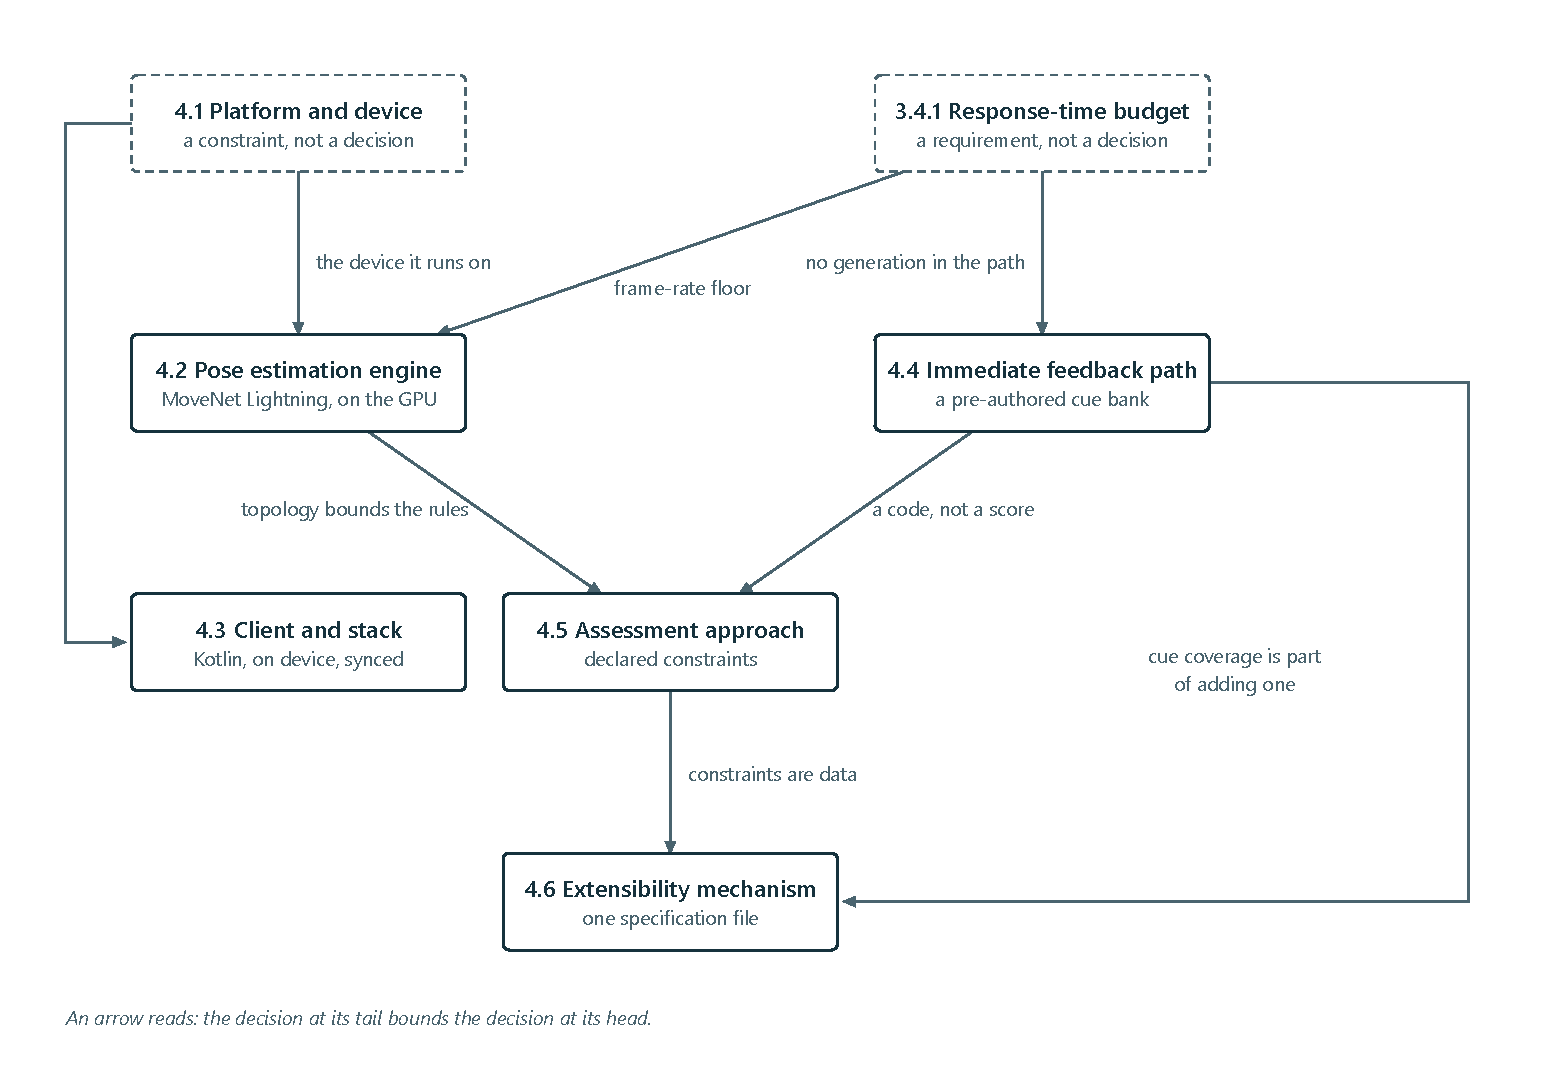
\includegraphics[width=\textwidth]{fig-4-1-decision-dependencies.pdf}
\caption[How the six design decisions constrain one another]{What constrains what. Dashed boxes are not decisions: one is a requirement and one is a constraint, and the chapter is ordered so that nothing is argued before the thing that bounds it.}
\label{fig:4.1}
\end{figure}

Two roots are not decisions. The response-time budget derived in 3.4.1 removes a language model from the live path in 4.4 and sets the frame-rate floor the engine is measured against in 4.2, and the handset in 4.1 is what every figure in the chapter is a figure about.

Three dependencies run in the direction a reader would not expect.

\textbf{The feedback path constrains the assessment layer rather than consuming whatever it produces.} Because the cue is a lookup on a discrete code, the assessment layer has to classify rather than score. A design emitting a continuous quality value would be reasonable in isolation and unusable here.

\textbf{The engine bounds the extensibility claim.} The format declares the landmarks an exercise depends on, so the set of exercises that can ever be declared is bounded by what the engine emits. The engine chosen in 4.2 stops at the ankle, so a future exercise whose fault needs the heel or the toe is not a specification away; it is an engine away.

\textbf{The engine's noise reaches the thresholds, which the arrows do not show.} A measurement noisier than the quantity being decided cannot support a threshold on it, so the number in 4.5.2 is a property of the engine in 4.2 as much as of the movement. 4.2.5 records the one place where that dependency was left implicit and failed silently.
